\section{Project Structure}
The software is divided into three main components: the robot behavior implementation, a custom lightweight 2D simulator, and a ROS 2-based 3D simulation environment. \Cref{fig:software-structure} shows the dependency structure of the \texttt{botbrain} behavior library and the two simulates which will be further explained in the following sections.

\begin{figure}[H]
    \begin{center}
        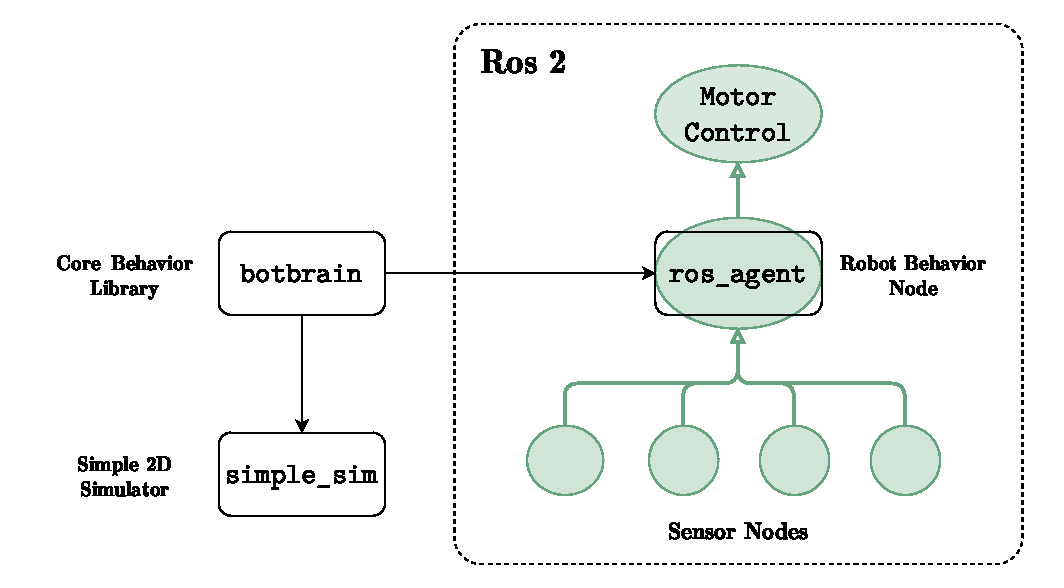
\includegraphics[width=0.95\textwidth]{figures/software-structure.pdf}
    \end{center}
    \caption{Software structure of the project. Black arrows indicate library dependencies, while green arrows denote ROS 2 communication through topics. Square boxes represent Rust crates and green circles represent ROS 2 nodes. The core library \texttt{botbrain} is ROS 2-independent and can be reused by the simple simulator without any dependency on ROS 2.}
    \label{fig:software-structure}
\end{figure}

\subsection{Simulated Hardware}
% TODO: Describe the robot we are designing for
% TODO: Describe the sensors available
% TODO: Describe that we assume the robot to have some sort of communication method

A simulated differential-drive robot equipped with a camera, LiDAR, odometry, and communication capabilities is used as the target platform. LiDAR and odometry are used for localization via Adaptive Monte Carlo Localization (AMCL), as discussed in \cref{sub:localization}. The camera is used for object detection, and a communication channel is assumed for data exchange between robots.\\

To ensure realism and leverage existing 3D models and URDF files, the Turtlebot 4 \cite{tb4} is selected as the simulated platform. Although the Turtlebot 4 lacks a dedicated communication unit, this project simulates inter-robot messaging, rendering the system agnostic to the specific communication method. The software can be adapted to any robot platform that satisfies the sensor and communication requirements by configuring parameters in the source code.

% TODO: Maybe mark the sensors on the robot
\begin{figure}[h]
    \begin{center}
        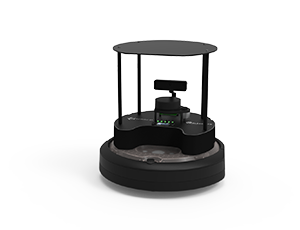
\includegraphics[width=0.55\textwidth]{figures/tb4.png}
    \end{center}
    \caption{Turtlebot 4 platform used in simulation.}
    \label{fig:tb4}
\end{figure}

% TODO: Where to put this??
\subsection{Using Rust}
% TODO: Describe how we integrated with colcon

The core of the system is implemented in Rust. While this choice was primarily based on developer preference, it brings several notable benefits. Although ROS 2 does not officially support Rust, the \texttt{r2r} library \cite{r2r} provides bindings to the ROS Client Library (RCL), enabling message serialization, topic publication/subscription, and integration with other ROS components. The initial build times are longer compared to C++, as Rust bindings are generated during compilation.\\

% TODO: Write about burn or do it in reinforcement learning section

Rust's memory safety guarantees and strong static typing contribute to a more robust and maintainable codebase. The compiler ensures that object lifetimes are correctly managed, eliminating an entire class of memory-related bugs. These features make Rust particularly well-suited for collaborative development, where code clarity and correctness are critical. \Cref{fig:simulators} shows screenshots of both simulators operating in the same map layout.

\subsection{Robot Behavior}
Robot behavior is implemented in the \texttt{botbrain} library, which defines a common \texttt{Robot} interface that exposes a robot’s internal state to external programs (see \cref{fig:robot-interface}).

\begin{figure}[H]
    \begin{center}
        \begin{minted}[autogobble]{rust}
            pub trait Robot {
                fn set_id(&mut self, id: RobotId);            // Set the ID of the robot
                fn set_map(&mut self, world: Map);            // Set the world map

                fn input_pose(&mut self, pose: RobotPose);    // Input the robot's pose
                fn input_cam(&mut self, cam: CamData);        // Input camera data
                fn input_lidar(&mut self, lidar: LidarData);  // Input LiDAR data
                fn input_msgs(&mut self, msgs: Vec<Message>); // Input messages from other robots

                fn get_id(&self) -> &RobotId;                 // Retrieve the robot's ID
                ...
            }
        \end{minted}
    \end{center}
    \caption{Methods of the \texttt{Robot} interface.}
    \label{fig:robot-interface}
\end{figure}

Methods prefixed with \texttt{set} are intended for initialization and must be called before any other interaction. The \texttt{input} methods are used to provide live sensor data and messages from other robots, while \texttt{get} methods retrieve state information without modifying it. Notably, the interface does not include a method that directly runs the robot’s control loop. Instead, the \texttt{Robot} represents only the internal state. Control logic is implemented as an external function that reads from and writes to this state to produce a control signals and a list of outbound messages. This separation allows for multiple behavior implementations to operate on the same robot state, simplifying algorithm comparison.

\subsection{Behavior Debugging}
To facilitate development and validation, the simple simulator supports real-time debugging of both robot behavior and internal state. The \texttt{botbrain} library exposes a debugging interface known as the \texttt{Debug Soup}, which allows behavior modules to annotate the simulation with structured debugging data. These debug items --- such as occupancy grids, path vectors, target points, and internal decision states --- can be visualized in both \texttt{simple\_sim} and ROS 2 via RViz2. The debug items are located on the right panel i the \texttt{simple\_sim} user interface as seen on \cref{fig:simple-sim-interface} and their overlays can be toggled at will. This significantly accelerates the development process and helps in interpreting the emergent behavior of the swarm. The \texttt{Debug Soup} can be disabled to save memory and increase performance after development is done.

\subsection{Two Simulators}
This project uses a simulator-to-simulator approach rather than attempting direct deployment to physical hardware. Two simulators were developed and used: a lightweight custom 2D simulator called \texttt{simple\_sim}, and a more realistic 3D simulation in Gazebo integrated with ROS 2. \\

The 2D simulator supports rapid prototyping, debugging, and algorithm iteration. It is deterministic, lightweight, and capable of much running faster than real time in most cases. The Gazebo simulation, by contrast, is much more computationally heavy and provides high-fidelity sensor emulation and more realistic robot dynamics. It is used to validate that behaviors developed in the simpler simulator transfer correctly to a close to real environment. \\

% Both simulators run identical robot behavior code using the shared \texttt{botbrain} library as shown in \cref{fig:software-structure}. This ensuring consistent robot behavior in both simulators.

% TODO: Insert pictures of the depot in Simple Sim and Gazebo
% TODO: Insert image of RViz2 and simple_sim side-by-side showing the same data
\begin{figure}[h]
    \centering
    \begin{subfigure}[b]{0.45\textwidth}
        \centering
        \includegraphics[width=\textwidth]{figures/simple_sim.png}
        \caption{Simple Simulator}
    \end{subfigure}
    \hfill
    \begin{subfigure}[b]{0.45\textwidth}
        \centering
        \includegraphics[width=\textwidth]{figures/gazebo_sim.png}
        \caption{Gazebo Simulator in ROS 2}
    \end{subfigure}
    \caption{Screenshots of the simulators running the "depot" environment.}
    \label{fig:simulators}
\end{figure}

The double simulator architecture is built around the shared \texttt{botbrain} behavior library, which encapsulates each robot’s internal state and provides a standardized interface for behavior control. This modular design allows the same behavior code to be executed seamlessly in both the lightweight \texttt{simple\_sim} environment and the more realistic Gazebo/ROS~2 simulation without requiring any code changes. By decoupling the behavior logic from the underlying simulation platform, the system supports consistent benchmarking and fair comparisons between algorithms. This separation also promotes cleaner, more testable, and reusable code, making it easier to iterate on behaviors and evaluate improvements.\\
